\documentclass[tikz, convert = false]{standalone}%

\usepackage[utf8]{inputenx}%  http://ctan.org/pkg/inputenx
% Euler for math | Palatino for rm | Helvetica for ss | Courier for tt
\renewcommand{\rmdefault}{ppl}% rm
\linespread{1.05}% Palatino needs more leading
\usepackage[scaled]{helvet}% ss //  http://ctan.org/pkg/helvet
\usepackage{courier}% tt // http://ctan.org/pkg/courier
\usepackage{eulervm}  %  http://ctan.org/pkg/eulervm
% a better implementation of the euler package (not in gwTeX)
\normalfont%
\usepackage[T1]{fontenc}%  http://ctan.org/pkg/fontenc
\usepackage{textcomp}%  http://ctan.org/pkg/textcomp

\usetikzlibrary{calc}
\usetikzlibrary{intersections}

\tikzset{Hidden Line/.style = {thin, gray!30}}

\begin{document}
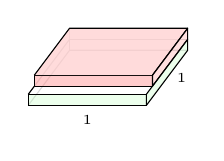
\begin{tikzpicture}[x =1 .5cm, y = 0.7cm]
  \coordinate (O) at (0, 0);
  \coordinate (P1) at (0.35, 1);
  \coordinate (P2) at (1.35, 1);
  \coordinate (P3) at (1, 0);

  \draw[Hidden Line] (O) -- (P1) -- (P2);

  \path (O) -- (P3) node[pos = .5, font = \tiny, below] {$1$};

  \draw [fill = green!25, fill opacity = 0.3] (O) -- +(0, .2) coordinate (P4) --
  +(1, .2) coordinate (P5) -- +(1, 0) -- cycle;

  \path  (P3) -- (P2) node[pos = .5, right, font = \tiny] {$1$};
  \path[name path = uil, red] (P5) -- ($(P2) + (0, .2)$) coordinate (P6) --
  +(0, -.2);

  \draw [fill = green!25, fill opacity = 0.3, join = round] ($(P3) +(0, 0.2)$) --
  (P3) -- (P2) -- ++(0, 0.2) -- cycle;

  \draw [Hidden Line] (P6) -- +(-1, 0) coordinate (P7);
  \draw [Hidden Line] (P7) -- (P1);

  \path[name path = uol] (P4) -- (P7);
  \path[name path = hl] (0, .35) -- +(1.25, 0);
  \path[name intersections = {of = uol and hl}];

  \coordinate (P8) at (intersection-1);

  \draw [Hidden Line] (P8) -- (P7);
  \draw  (P8) -- (P4);

  \path[name intersections = {of = uil and hl}];

  \coordinate (P9) at (intersection-1);

  \path  (P6) -- +(0, .2) coordinate (P12);
  \coordinate (P13) at ($(P12)+(-1, 0)$);
  \draw[Hidden Line, draw opacity = 0.8] (P13) -- +(0, -.2);

  \draw [fill = red!40, fill opacity = 0.5] (P9) -- (P8) -- +(0, .2) coordinate
  (P10) -- +(1, .2) coordinate (P11) -- (P9);

  \draw [fill = red!20, fill opacity = 0.7, join = round] (P11) -- (P12) --
  (P13) -- (P10);

  \draw [fill = red!60, fill opacity = 0.2, join = round] (P6) -- ++(0, .2) --
  (P11) -- ++(0, -.2) -- cycle;
\end{tikzpicture}
\end{document}